\needspace{10\baselineskip}
\section{Visualização de dados com Matplotlib}
\label{sec:visualizacao}

O tipo de gráfico depende da pergunta. Linhas mostram mudanças ao longo do tempo. Barras comparam categorias. Histogramas e boxplots descrevem a distribuição de uma variável numérica. A dispersão mostra a relação entre duas variáveis numéricas \cite{matplotlib}.

\subsection{Figura, eixos e rótulos}

\codigo{plt.subplots()} cria a figura (\codigo{fig}) e os eixos (\codigo{ax}). A figura é a área completa. Cada conjunto de eixos é um painel onde são desenhados dados, rótulos e marcas de escala. O argumento \codigo{figsize} define largura e altura em polegadas. \codigo{ax.set()} reúne ajustes de título e rótulos, e \codigo{plt.show()} exibe o resultado.

Nos exemplos com notas, \codigo{df\_validas} é a tabela criada na Seção \ref{sec:ausentes}. Ela reúne os \(16\) registros com nota observada.

\needspace{33\baselineskip}
\subsection{Gráfico de linhas}

\codigo{ax.plot(x, y)} liga os pontos na ordem em que os dados são fornecidos. Aqui, cada posição em \codigo{dias} corresponde à quantidade de vendas na mesma posição de \codigo{vendas}. \codigo{marker="o"} marca os valores observados. A linha tracejada representa uma meta de \(12\) vendas.

Entre dois pontos consecutivos \((x_i,y_i)\) e \((x_{i+1},y_{i+1})\), com dias distintos, o segmento tem inclinação
\[
  m_i=\frac{y_{i+1}-y_i}{x_{i+1}-x_i}.
\]
Do dia \(2\) ao dia \(3\), a inclinação é \((8-12)/(3-2)=-4\) vendas por dia. O sinal indica que a linha desce nesse intervalo.

\begin{exemplo}
import matplotlib.pyplot as plt

dias = [1, 2, 3, 4, 5]
vendas = [10, 12, 8, 15, 18]

fig, ax = plt.subplots(figsize=(6.3, 3.5), layout="constrained")
ax.plot(dias, vendas, marker="o", color="#19476B", label="Vendas")
ax.axhline(12, linestyle="--", color="#67747C", label="Meta")
ax.set(title="Vendas por dia", xlabel="Dia",
       ylabel="Vendas (unidades)", xticks=dias)
ax.legend(frameon=False)
plt.show()
\end{exemplo}

\noindent\begin{minipage}{\linewidth}
\centering
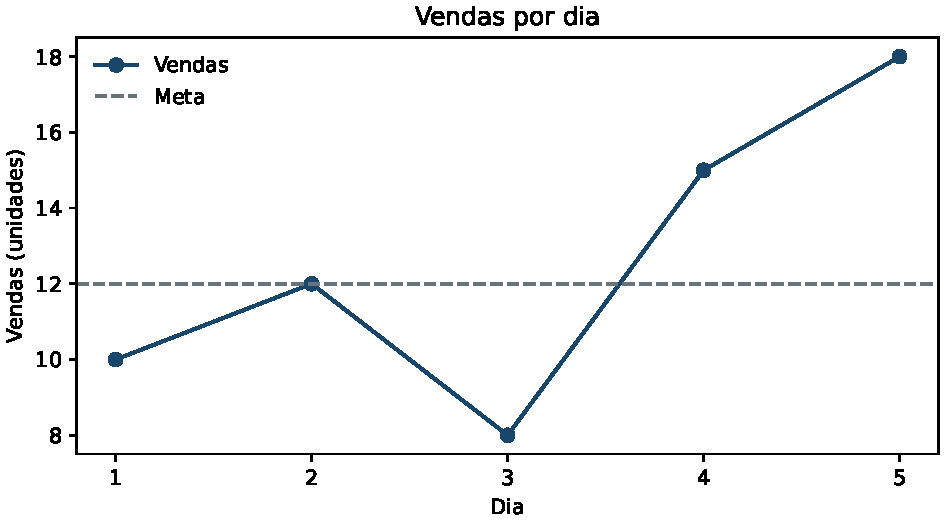
\includegraphics[width=0.76\linewidth]{figuras/linhas.pdf}

\raggedright
As vendas caem de \(12\) para \(8\) entre o segundo e o terceiro dia e voltam a subir até \(18\) no quinto. Os pontos mostram as contagens observadas em cada dia.
\end{minipage}

\needspace{33\baselineskip}
\subsection{Legendas para identificar as séries}
\label{sec:legendas}

Em um gráfico com várias séries, o argumento \codigo{label} dá um nome a cada série. A chamada a \codigo{ax.legend()} após o desenho das séries exibe esses nomes. A legenda usa esses nomes junto com a cor, o marcador e o estilo da linha de cada série \cite{matplotlib}.

\begin{exemplo}
import matplotlib.pyplot as plt

dias = [1, 2, 3, 4, 5]
loja_a = [10, 12, 8, 15, 18]
loja_b = [8, 9, 11, 13, 15]

fig, ax = plt.subplots(figsize=(6.3, 3.5), layout="constrained")
ax.plot(dias, loja_a, label="Loja A", marker="o", color="#19476B")
ax.plot(dias, loja_b, label="Loja B", marker="s",
        linestyle="--", color="#A45727")
ax.set(title="Vendas por loja", xlabel="Dia",
       ylabel="Vendas (unidades)", xticks=dias)
ax.legend(title="Loja", loc="upper left", frameon=False)
plt.show()
\end{exemplo}

\noindent\begin{minipage}{\linewidth}
\centering
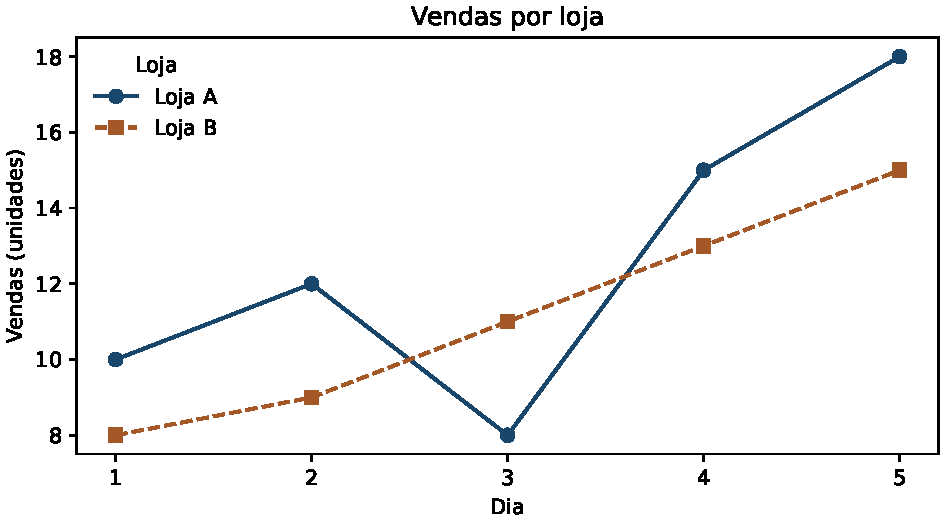
\includegraphics[width=0.76\linewidth]{figuras/legendas.pdf}

\raggedright
A linha contínua representa a Loja A e a tracejada representa a Loja B. No dia \(3\), a Loja B vendeu \(11\) unidades e a Loja A vendeu \(8\).
\end{minipage}

O argumento \codigo{title} dá um título à legenda. \codigo{loc="upper left"} posiciona a legenda no canto superior esquerdo. Se essa posição cobrir dados importantes, outra posição pode ser indicada. Com \codigo{loc="best"}, o Matplotlib escolhe entre as posições disponíveis.

\needspace{33\baselineskip}
\subsection{Gráfico de barras}

\codigo{ax.bar()} recebe as categorias e suas alturas. Neste exemplo, as alturas são as contagens de notas válidas por curso, obtidas com \codigo{value\_counts()}. A base zero permite comparar as alturas diretamente. Se \(c_i\) é o curso do registro \(i\) com nota válida, a altura da barra do curso \(c\) é
\[
  h_c=\sum_{i=1}^{n}\mathbf{1}(c_i=c).
\]
A função indicadora \(\mathbf{1}\) vale \(1\) quando a condição é verdadeira e \(0\) nos demais casos. A soma conta os registros que pertencem ao curso.

\begin{exemplo}
import matplotlib.pyplot as plt
from matplotlib.ticker import MaxNLocator

contagens = df_validas["curso"].value_counts().sort_index()

fig, ax = plt.subplots(figsize=(6.3, 3.5), layout="constrained")
barras = ax.bar(contagens.index, contagens.values, color="#19476B")
ax.set(title="Notas observadas por curso", xlabel="Curso",
       ylabel="Quantidade de notas", ylim=(0, 7))
ax.yaxis.set_major_locator(MaxNLocator(integer=True))
ax.bar_label(barras, padding=3)
plt.show()
\end{exemplo}

\noindent\begin{minipage}{\linewidth}
\centering
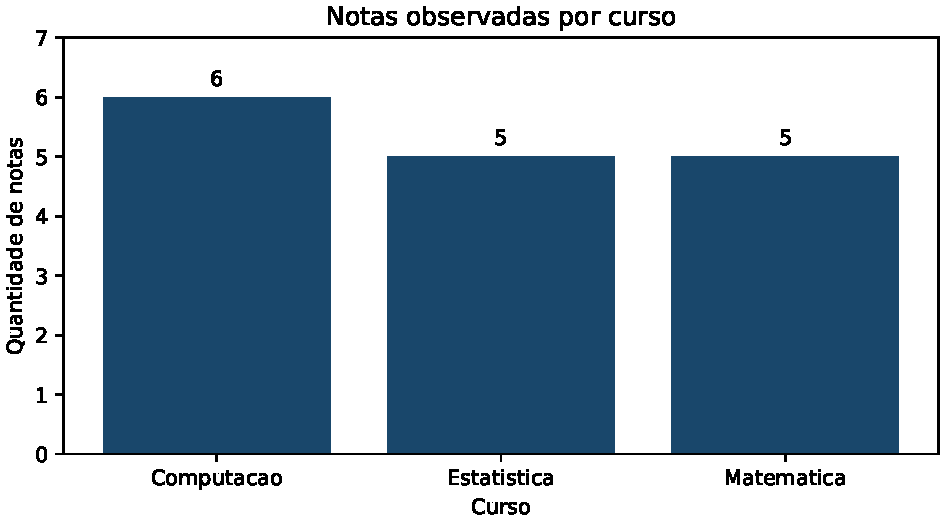
\includegraphics[width=0.76\linewidth]{figuras/barras.pdf}

\raggedright
Computação tem seis notas disponíveis. Estatística e Matemática têm cinco cada. Como a base original tem seis registros por curso, o gráfico ajuda a identificar onde há notas ausentes.
\end{minipage}

\needspace{33\baselineskip}
\subsection{Histograma}

O histograma resume uma variável numérica agrupando seus valores em intervalos. \codigo{ax.hist()} recebe as observações e usa \codigo{bins} para definir os intervalos. Um inteiro, como \codigo{bins=5}, pede cinco intervalos de mesma largura na faixa dos dados. Uma lista fornece os limites explicitamente. Com \codigo{[5, 6, 7, 8, 9, 10]}, os cinco intervalos têm largura \(1\).

Os intervalos incluem o limite esquerdo e excluem o direito. O último também inclui o limite direito. Assim, uma nota \(8{,}0\) entra no intervalo de \(8\) a \(9\), e uma nota \(10{,}0\) entraria no último \cite{matplotlib}.

Para notas \(x_1,\ldots,x_n\) e um intervalo \([b_j,b_{j+1})\), a altura em contagens é \(n_j\) e a frequência relativa é \(f_j\):
\[
  n_j=\sum_{i=1}^{n}\mathbf{1}(b_j\le x_i<b_{j+1}),
  \qquad f_j=\frac{n_j}{n}.
\]
No último intervalo, a desigualdade superior inclui o valor \(b_{j+1}\). No gráfico abaixo, o eixo vertical mostra \(n_j\).

\begin{exemplo}
import matplotlib.pyplot as plt
from matplotlib.ticker import MaxNLocator

notas = df_validas["nota"]
limites = [5, 6, 7, 8, 9, 10]

fig, ax = plt.subplots(figsize=(6.3, 3.5), layout="constrained")
alturas, _, _ = ax.hist(notas, bins=limites,
                       color="#19476B", edgecolor="white")
ax.set(title="Histograma das notas", xlabel="Nota",
       ylabel="Contagem", xticks=limites)
ax.yaxis.set_major_locator(MaxNLocator(integer=True))
print(alturas.astype(int).tolist())  # [2, 3, 4, 4, 3]
plt.show()
\end{exemplo}

\noindent\begin{minipage}{\linewidth}
\centering
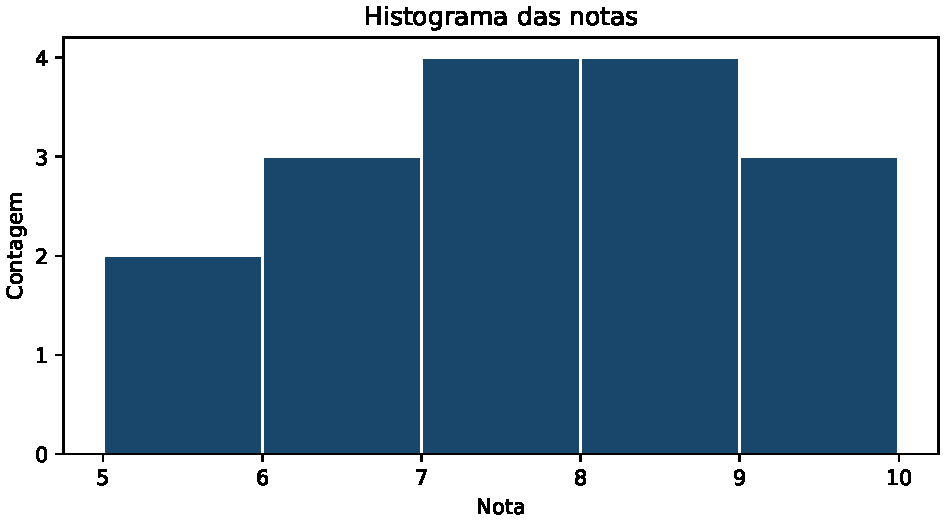
\includegraphics[width=0.76\linewidth]{figuras/distribuicao.pdf}

\raggedright
O gráfico tem quatro notas de \(7\) a menos de \(8\) e outras quatro de \(8\) a menos de \(9\). Cada intervalo contém \(4/16=25\%\) das notas observadas, e os dois juntos concentram \(50\%\).
\end{minipage}

A largura dos intervalos muda o que fica visível. Com poucos intervalos, detalhes podem ser agregados. Com muitos, uma base pequena pode produzir várias barras vazias. Ao comparar dois histogramas, usar os mesmos limites facilita a leitura. Valores fora desses limites ficam de fora do gráfico. Se \(n\) continua sendo o total original, as frequências \(n_j/n\) podem somar menos de \(100\%\).

\needspace{33\baselineskip}
\subsection{Boxplot}

\codigo{ax.boxplot()} resume a distribuição de uma variável. A caixa vai do primeiro ao terceiro quartil, e a linha dentro dela marca a mediana. Com a configuração padrão, os bigodes chegam até as observações mais extremas dentro dos limites de \(1{,}5\) vez o intervalo interquartil. Pontos além dos bigodes aparecem separadamente \cite{matplotlib}. Com \(Q_1\) e \(Q_3\) como limites da caixa, os limites para localizar os bigodes são
\[
  \mathrm{IQR}=Q_3-Q_1,\qquad
  L=Q_1-1{,}5\,\mathrm{IQR},\qquad U=Q_3+1{,}5\,\mathrm{IQR}.
\]
No exemplo, \(\mathrm{IQR}=8{,}50-6{,}625=1{,}875\). Os bigodes chegam às observações extremas dentro de \([L,U]\).

\begin{exemplo}
import matplotlib.pyplot as plt

notas = df_validas["nota"]

fig, ax = plt.subplots(figsize=(6.3, 3.4), layout="constrained")
ax.boxplot(notas, widths=0.4,
           medianprops={"color": "#19476B", "linewidth": 2})
ax.set(title="Boxplot das notas", ylabel="Nota", xticks=[])
plt.show()
\end{exemplo}

\noindent\begin{minipage}{\linewidth}
\centering
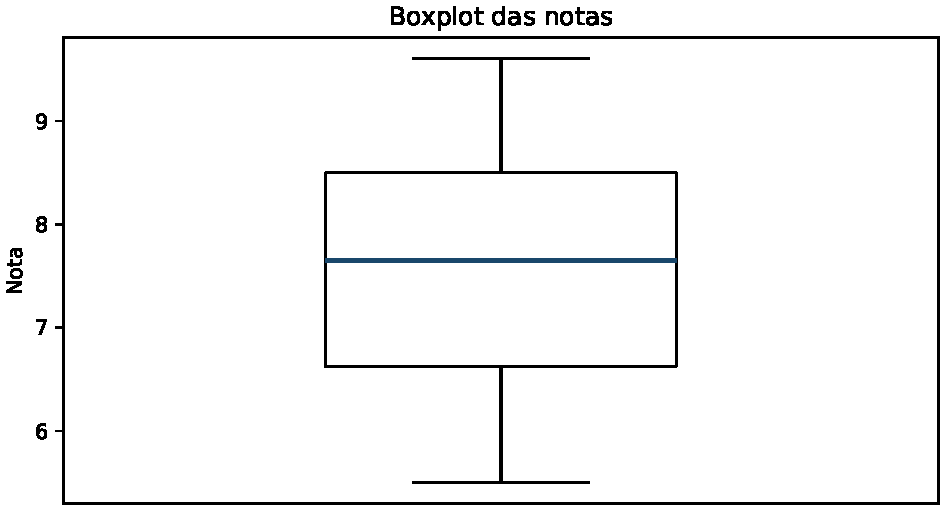
\includegraphics[width=0.76\linewidth]{figuras/boxplot.pdf}

\raggedright
A mediana é \(7{,}65\). A caixa delimita a metade central dos dados, entre \(6{,}625\) e \(8{,}50\). Neste caso, nenhuma observação fica além dos bigodes.
\end{minipage}

\needspace{33\baselineskip}
\subsection{Gráfico de dispersão}

\codigo{ax.scatter(x, y)} desenha um ponto para cada par de valores. No exemplo, cada ponto representa um participante. A coordenada horizontal indica horas de estudo e a vertical indica nota. O filtro de notas válidas é aplicado antes de selecionar as duas colunas para preservar o pareamento. O primeiro participante, por exemplo, aparece no ponto \((2,\;5{,}9)\). A correlação de Pearson resume a associação linear dos pares \((x_i,y_i)\):
\[
  r=\frac{\sum_i(x_i-\bar x)(y_i-\bar y)}
          {\sqrt{\sum_i(x_i-\bar x)^2}\,\sqrt{\sum_i(y_i-\bar y)^2}}.
\]
\(\bar x\) e \(\bar y\) são as médias das horas de estudo e das notas, respectivamente.

\begin{exemplo}
import matplotlib.pyplot as plt

fig_dispersao, ax = plt.subplots(figsize=(6.3, 3.6), layout="constrained")
ax.scatter(df_validas["horas_estudo"], df_validas["nota"],
           color="#19476B", alpha=0.85)
ax.set(title="Horas de estudo e nota",
       xlabel="Horas de estudo (h)", ylabel="Nota")
ax.set_axisbelow(True)
ax.grid(alpha=0.2)

r = df_validas["horas_estudo"].corr(df_validas["nota"])
print(round(r, 2))  # 0.96
plt.show()
\end{exemplo}

\noindent\begin{minipage}{\linewidth}
\centering
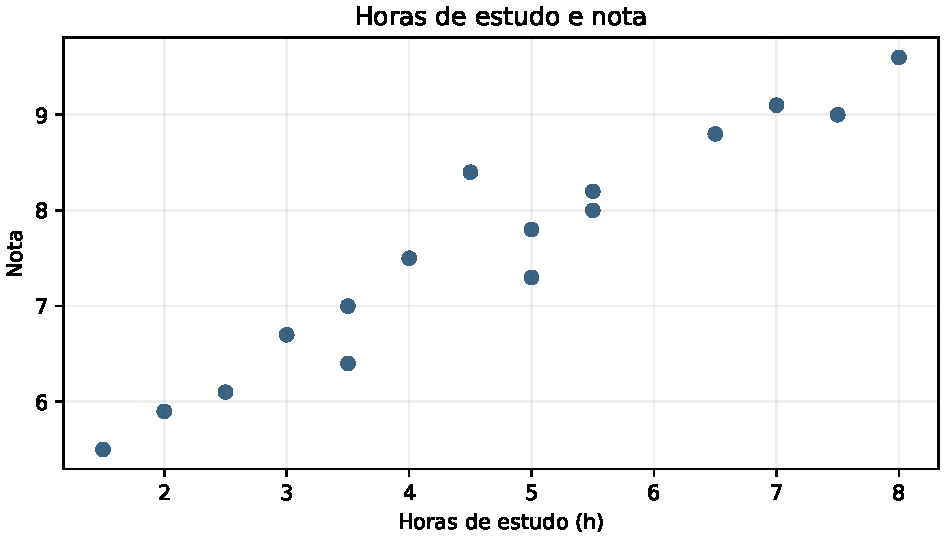
\includegraphics[width=0.62\linewidth]{figuras/dispersao.pdf}

\raggedright
A tendência ascendente e \(r=0{,}96\) indicam associação linear positiva na base simulada. Esse resultado, sozinho, é insuficiente para estabelecer causalidade.
\end{minipage}

\subsection{Salvar figuras}

\codigo{fig\_dispersao.savefig()} salva a figura de dispersão mesmo após a criação de outros gráficos. A extensão define o formato: PNG para imagem em pixels e PDF para preservar elementos vetoriais.

\begin{exemplo}
fig_dispersao.savefig("dispersao.png", dpi=200, bbox_inches="tight")
fig_dispersao.savefig("dispersao.pdf", bbox_inches="tight")
\end{exemplo}

Em scripts, a gravação pode preceder \codigo{plt.show()}. No Colab, os arquivos ficam no painel \textbf{Arquivos}.
